\chapter{Statistics}
\begin{exercises}{}{
    \begin{enumerate}[noitemsep, label=\textbf{\arabic*}.]
%question1
    \item Calculate the mean, median and mode of the following data sets:
      \begin{enumerate}[noitemsep, label=\textbf{(\alph*)} ]
      \item $2;~5;~8;~8;~11;~13;~22;~23;~27$
      \item $15;~17;~24;~24;~26;~28;~31;~43$
      \item $4;~11;~3;~15;~11;~13;~25;~17;~2;~11$
      \item $24;~35;~28;~41;~32;~49;~31$
      \end{enumerate}
%question2
    \item The ages of $15$ runners of the Comrades Marathon were recorded:
      \begin{equation*}
        31;~42;~28;~38;~45;~51;~33;~29;~42;~26;~34;~56;~33;~46;~41
      \end{equation*}
      Calculate the mean, median and modal age.
%question3
    \item In the first of a series of jars, there is $1$ sweet. In the
      second jar, there are $3$ sweets. The mean number of sweets in the
      first two jars is $2$.
      \begin{enumerate}[noitemsep, label=\textbf{(\alph*)} ]
      \item If the mean number of sweets in the first three jars is $3$, how
        many sweets are there in the third jar?
      \item If the mean number of sweets in the first four jars is $4$, how
        many sweets are there in the fourth jar?
      \end{enumerate}
%question4
    \item Find a set of five ages for which the mean age is $5$, the modal
      age is $2$ and the median age is $3$ years.
%question5
    \item Four friends each have some marbles. They work out that the mean
      number of marbles they have is $10$. One friend leaves with $4$
      marbles. How many marbles do the remaining friends have together?
\end{enumerate}
}
\end{exercises}


 \begin{solutions}{}{
\begin{enumerate}[itemsep=5pt, label=\textbf{\arabic*}. ] 


\item %solution1
      \begin{enumerate}[noitemsep, label=\textbf{(\alph*)} ]
\item Mean $= 13,2$; ~Median $= 11$;~ Mode $= 8$ %$2;~5;~8;~8;~11;~13;~22;~23;~27$
\item Mean $= 26$;~ Median $= 25$; ~Mode $= 24$%$15;~17;~24;~24;~26;~28;~31;~43$
\item Mean $=11,2$; ~Median $= 11$;~ Mode $=11$%$4;~11;~3;~15;~11;~13;~25;~17;~2;~11$
\item Mean $=34,29$; ~Median $=32$;~ No mode%$24;~35;~28;~41;~32;~49;~31$
    \end{enumerate}
\item %solution2
Mean $=38,3$; Median $= 38$; Mode $= 33$ and $42$\\
\item %solution3
       \begin{enumerate}[noitemsep, label=\textbf{(\alph*)} ]
\item Let $n_3$ be the number of sweets in the third jar:\\
$\frac{1+3+n_3}{3}=3\\
1+3+n_3=9\\
n_3=5$\\

\item Let $n_4$ be the number of sweets in the fourth jar:\\
$\frac{1+3+5+n_4}4=4\\
9+n_4=16\\
n_4=7$
    \end{enumerate}

\item %solution 4
Let the five different ages be $x_1,~x_2,~x_3,~x_4$ and $x_5$.\\
Therefore the mean is\\

$\frac{x_1+x_2+x_3+x_4+x_5}{5}=5\\
x_1+x_2+x_3+x_4+x_5=25\\$
 
The median value is at position $3$, therefore $x_3=3$.\\

The mode is the age that occurs most often. There are at least $2$ ages to be $2$. The other ages would all have to be different. The four unknown ages can't all be $2$, as that would not give us a mean of $5$. Also since all calculations of mean, mode and median are done on ordered sets of data we can't have $3$ ages being $2$, because then the median age would not be $3$. So we have \\

$2+2+3+x_4+x_5=25\\
18=x_4+x_5$\\

$x_4$ and $x_5$ can be any numbers that add up to $18$ and are not the same, so $12$ and $6$ or $8$ and $10$ or $3$ and $15$, etc.\\

Possible data sets:\\
$2, 2, 3, 3, 15; ~~
2, 2, 3, 4, 14; ~~ 
2, 2, 3, 5, 13; ~~ 
2, 2, 3, 6, 12; ~~
2, 2, 3, 7, 11; ~~ 
2, 2, 3, 8, 10$\\

Note that the set of ages must be ordered, the median value must be $3$ and there must be $2$ ages of $2$.\\


\item %solution 5
Let the number of marbles per friend be $x_1,~x_2,~x_3 $ and $ x_4$.\\
$\frac{x_1+x_2+x_3+x_4}{4}=10\\
x_1+x_2+x_3+x_4=40$\\
One friend leaves, \\
$x_1+x_2+x_3=40−4\\
x_1+x_2+x_3=36$\\

Therefore the remaining friends have $36$ marbles.

\end{enumerate}}
\end{solutions}

\begin{exercises}{}{
    \begin{enumerate}[itemsep=5pt, label=\textbf{\arabic*}. ]
    \item  A class experiment was conducted and $50$ learners were asked to
      guess the number of sweets in a jar. The following guesses were
      recorded:
      \\
      \begin{center}
        \begin{tabular}{|c|c|c|c|c|c|c|c|c|c|} \hline
          56 & 49 & 40 & 11 & 33 & 33 & 37 & 29 & 30 & 59 \\ \hline
          21 & 16 & 38 & 44 & 38 & 52 & 22 & 24 & 30 & 34 \\\hline
          42 & 15 & 48 & 33 & 51 & 44 & 33 & 17 & 19 & 44 \\\hline
          47 & 23 & 27 & 47 & 13 & 25 & 53 & 57 & 28 & 23 \\\hline
          36 & 35 & 40 & 23 & 45 & 39 & 32 & 58 & 22 & 40 \\\hline
        \end{tabular}
      \end{center}
      \begin{enumerate}[noitemsep, label=\textbf{(\alph*)} ]
      \item
        Draw up a grouped frequency table using the intervals\\
        $10 < x \leq 20$;\ $20 < x \leq 30$;\ $30 < x \leq 40$;\ 
        $40 < x \leq 50$; and \ $50 < x \leq 60$.
      \item Draw the histogram corresponding to the frequency table of the
        grouped data.
      \end{enumerate}
    \end{enumerate}
}
\end{exercises}


 \begin{solutions}{}{
\begin{enumerate}[itemsep=6pt, label=\textbf{\arabic*}. ] 
\item
%  Draw up a grouped frequency table using the intervals
%   $10 < x \leq 20$;\ $20 < x \leq 30$;\ $30 < x \leq 40$;\ 
%   $40 < x \leq 50$;and \ $50 < x \leq 60$.
\begin{enumerate}[itemsep=6pt, label=\textbf{(\alph*)} ]
% \begin{center}
\item 
\scalebox{1}{
  \begin{tabular}{|c|c|}\hline
\textbf{Group} & \textbf{Freq} \\ \hline
$11 - 20$ &$6$\\\hline
$21 - 30$&$13$\\\hline
$31 - 40$&$15$\\\hline
$41 - 50$&$9$\\\hline
$51 - 60$&$7$\\\hline
   
  \end{tabular}}

% \end{center}

\item %Draw the histogram corresponding to the frequency table of the   grouped data.
\scalebox{0.8} % Change this value to rescale the drawing.
{
\begin{pspicture}(0,-5.0875)(8.385716,5.0475)
\definecolor{color5165b}{rgb}{0.7725490196078432,0.7725490196078432,0.7725490196078432}
\rput(1.385716,-3.9525){\psaxes[linewidth=0.028222222,arrowsize=0.05291667cm 2.0,arrowlength=1.4,arrowinset=0.4,tickstyle=bottom,ticksize=0.10583333cm,dx=1.0cm,dy=1.0cm,Dx=10,Dy=2]{<->}(0,0)(-1,-1)(7,8)}
\psframe[linewidth=0.02,dimen=outer,fillstyle=solid,fillcolor=color5165b](3.3998826,0.0475)(2.3798826,-3.9490623)
\psframe[linewidth=0.02,dimen=outer,fillstyle=solid,fillcolor=color5165b](4.419883,2.6675)(3.3798826,-3.9490623)
\psframe[linewidth=0.02,dimen=outer,fillstyle=solid,fillcolor=color5165b](5.419883,3.6075)(4.379883,-3.9490623)
\psframe[linewidth=0.02,dimen=outer,fillstyle=solid,fillcolor=color5165b](6.399883,0.6875)(5.379883,-3.9490623)
\psframe[linewidth=0.02,dimen=outer,fillstyle=solid,fillcolor=color5165b](7.399883,-0.4125)(6.379883,-3.9490623)
% \usefont{T1}{ptm}{m}{n}
\rput(4.9245706,-4.8625){\LARGE Range of guesses}
% \usefont{T1}{ptm}{m}{n}
\rput{89.854546}(0.62033606,0.27754468){\rput(0.13573046,0.46597877){\LARGE Count}}
\end{pspicture} 
}
\end{enumerate}
\end{enumerate}}
\end{solutions}


\begin{exercises}{}{
  \begin{enumerate}[itemsep=8pt, label=\textbf{\arabic*}.]
%question1
 \item Consider the following grouped data and calculate the mean,
    the modal group and the median group.
\\
    \begin{center}
      \begin{tabular}{|c|c|}\hline
        \textbf{Mass (kg)} & \textbf{Count} \\\hline
        $40 < m \leq 45$ & $7$ \\\hline
        $45 < m \leq 50$ & $10$ \\\hline
        $50 < m \leq 55$ & $15$ \\\hline
        $55 < m \leq 60$ & $12$ \\\hline
        $60 < m \leq 65$ & $6$ \\\hline
      \end{tabular}
    \end{center}
%question2
\item Find the mean, the modal group and the median group in this
    data set of how much time people needed to complete a game.
\\
    \begin{center}
      \begin{tabular}{|c|c|} \hline
       \textbf{Time (s)} & \textbf{Count} \\ \hline
        $35 < t \leq 45$ & $5$ \\\hline
        $45 < t \leq 55$ & $11$ \\\hline
        $55 < t \leq 65$ & $15$ \\\hline
        $65 < t \leq 75$ & $26$ \\\hline
        $75 < t \leq 85$ & $19$ \\\hline
        $85 < t \leq 95$ & $13$ \\\hline
        $95 < t \leq 105$ & $6$ \\\hline
      \end{tabular}
    \end{center}
%question3
\item The histogram below shows the number of passengers that travel in Alfred's minibus taxi per week.\\
Calculate
\begin{enumerate}[noitemsep, label=\textbf{(\alph*)} ]
\item the modal interval
\item the total number of passengers to travel in Alfred's taxi
\item an estimate of the mean
\item an estimate of the median
\item if it is estimated that every passenger travelled an average distance of $5$ km, how much money would Alfred have made if he charged R~$3,50$ per km?
\end{enumerate}
\begin{center}
\scalebox{1} % Change this value to rescale the drawing.
{
\begin{pspicture}(0,-5.1475)(9.378126,5.1075)
\definecolor{color5165b}{rgb}{0.7725490196078432,0.7725490196078432,0.7725490196078432}
\rput(1.3781264,-3.8925){\psaxes[linewidth=0.028222222,arrowsize=0.05291667cm 2.0,arrowlength=1.4,arrowinset=0.4,tickstyle=bottom,ticksize=0.10583333cm,dx=1.0cm,dy=1.0cm,Dx=100,Dy=2,Ox=300]{<->}(0,0)(-1,-1)(8,9)}
\psframe[linewidth=0.02,dimen=outer,fillstyle=solid,fillcolor=color5165b](3.392293,-1.8890625)(2.372293,-3.8890624)
\psframe[linewidth=0.02,dimen=outer,fillstyle=solid,fillcolor=color5165b](4.412293,-0.8890625)(3.372293,-3.8890624)
\psframe[linewidth=0.02,dimen=outer,fillstyle=solid,fillcolor=color5165b](5.412293,2.1309376)(4.372293,-3.8890624)
\psframe[linewidth=0.02,dimen=outer,fillstyle=solid,fillcolor=color5165b](6.392293,4.1309376)(5.372293,-3.8890624)
\psframe[linewidth=0.02,dimen=outer,fillstyle=solid,fillcolor=color5165b](7.392293,0.1309375)(6.372293,-3.8890624)
\psframe[linewidth=0.02,dimen=outer,fillstyle=solid,fillcolor=color5165b](8.392293,-2.8690624)(7.372293,-3.8890624)
\rput(5.369637,-4.9225){No. of passengers}
\rput{89.854546}(0.73185694,0.38878262){\rput(0.13573053,0.5775){Count}}
\end{pspicture} 
}
\end{center}
  \end{enumerate}
}
\end{exercises}


 \begin{solutions}{}{
\begin{enumerate}[itemsep=5pt, label=\textbf{\arabic*}. ] 


\item Mean=$53$; Modal group: $50<m \leq 55$; Median group: $50 < m \leq 55$
\item Mean=$71,66$; Modal group: $65 < t \leq 75$; Median group: $65 < t \leq 75$
\item
\begin{enumerate}[noitemsep, label=\textbf{(\alph*)} ]
\item $700 < x\leq800$%the modal interval
\item $33~600$%the total number of passengers to travel in Alfred's taxi
\item $700$ %an estimate of the mean
\item $750$%an estimate of the median
\item R $588~ 000$%if it is estimated that every passenger travelled an average distance of $5$ km, how much money would Alfred have made if he charged R~$3,50$ per km?
\end{enumerate}
\end{enumerate}}
\end{solutions}

\begin{exercises}{}{
  \begin{enumerate}[noitemsep, label=\textbf{\arabic*}.]
%question1  
\item Find the range of the data set
    \begin{equation*}
      \{1;\ 2;\ 3;\ 4;\ 4;\ 4;\ 5;\ 6;\ 7;\ 8;\ 8;\ 9;\ 10;\ 10\}
    \end{equation*}
%question2    
\item What are the quartiles of this data set?
    \begin{equation*}
      \{3;\ 5;\ 1;\ 8;\ 9;\ 12;\ 25;\ 28;\ 24;\ 30;\ 41;\ 50\}
    \end{equation*}
%question3
  \item A class of $12$ students writes a test and the results are as
    follows:
    \begin{equation*}
      20;\ 39;\ 40;\ 43;\ 43;\ 46;\ 53;\ 58;\ 63;\ 70;\ 75;\ 91
    \end{equation*}
    Find the range, quartiles and the interquartile range.
%question4  
 \item Three sets of data are given:
    \begin{itemize}  
    \item \textbf{Data set 1:} $\{9;\ 12;\ 12;\ 14;\ 16;\ 22;\ 24\}$
    \item \textbf{Data set 2:} $\{7;\ 7;\ 8;\ 11;\ 13;\ 15;\ 16;\ 16\}$
    \item \textbf{Data set 3:} $\{11;\ 15;\ 16;\ 17;\ 19;\ 19;\ 22;\ 24;\ 27\}$
    \end{itemize}
    For each data set find:
    \begin{enumerate}[noitemsep, label=\textbf{(\alph*)} ]
    \item the range
    \item the lower quartile
    \item the interquartile range
    \item the semi-interquartile range
    \item the median
    \item the upper quartile
    \end{enumerate}
  \end{enumerate}
}
\end{exercises}


 \begin{solutions}{}{
\begin{enumerate}[itemsep=5pt, label=\textbf{\arabic*}. ] 
\item Range: $10-1=9$
\item $Q_1 = 6,2$;~ $ Q_2 = 18$;~ $Q_3 = 29$
\item Range: $91-20=71$\\
 $Q_1 = 41,5$; $Q_2 = 49,5$; $Q_3 = 66,5$ \\
 Interquartile range: $66,5-41,5=25$
\item 
\begin{enumerate}[noitemsep, label=\textbf{(\alph*)} ]
    \item Range: $24-9=15$; $~~16-7=9$; $~~27-11=16$
    \item $Q_1$: $12$;  $7,5$; $15,5$ 
    \item Interquartile range: $10$; $8$; $7,5$
    \item Semi-interquartile range: $5$; $4$; $3,75$
    \item Median: $14$; $12$; $19$
    \item $Q_3$: $22$; $15,5$; $23$
\end{enumerate}

\end{enumerate}}
\end{solutions}

\begin{exercises}{}{
    \begin{enumerate} [itemsep=6pt, label=\textbf{\arabic*}.]
%question1    
\item Lisa is working in a computer store. She sells the following
      number of computers each month:
      \begin{equation*}
        \{27;\ 39;\ 3;\ 15;\ 43;\ 27;\ 19;\ 54;\ 65;\ 23;\ 45;\ 16\}
      \end{equation*}
      Give the five number summary and box-and-whisker plot of Lisa's
      sales.
%question2      
\item Zithulele works as a telesales person. He keeps a record of the
      number of sales he makes each month. The data below show how much he
      sells each month.
      \begin{equation*}
        \{49;\ 12;\ 22;\ 35;\ 2;\ 45;\ 60;\ 48;\ 19;\ 1;\ 43;\ 12\}
      \end{equation*}
      Give the five number summary and box-and-whisker plot of Zithulele's
      sales.
%question3      
\item Hannah has worked as a florist for nine months. She sold the
      following number of wedding bouquets:
      \begin{equation*}
        \{16;\ 14;\ 8;\ 12;\ 6;\ 5;\ 3;\ 5;\ 7\}
      \end{equation*}
      Give the five number summary of Hannah's sales.
%question4      
\item Use the diagram below to determine the five number summary:
      \begin{enumerate}[noitemsep, label=\textbf{(\alph*)} ]
      \item 
    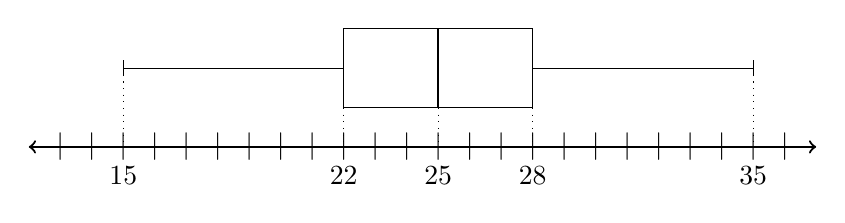
\begin{tikzpicture}[xscale=0.4]
      \def\median{25}
      \def\firstquartile{22}
      \def\thirdquartile{28}
      \def\minimum{15}
      \def\maximum{35}
      \draw (\firstquartile, -0.5 ) rectangle ( \thirdquartile,0.5);
      \draw[thick] ( \median,-0.5) -- ( \median,0.5);
      \draw (    \firstquartile, 0) -- (\minimum,0   );
      \draw ( \minimum, -0.1) -- (       \minimum, 0.1);
      \draw (  \thirdquartile, 0) -- (   \maximum, 0);
      \draw ( \maximum, -0.1) -- (      \maximum, 0.1 );
      \draw[thick,<->] (12,-1) -- (37,-1);
      \foreach \x in {\minimum, \firstquartile, \median, \thirdquartile, \maximum} {
        \draw (\x,-1.6) -- (\x, -1.6) node[anchor=south] {$\x$};
      }
      \foreach \x in {13,14,...,36} {
        \draw (\x,-1.3) -- (\x, -1.3) node[anchor=south] {$|$};
      }
      \draw[dotted] ( \maximum, 0) -- ( \maximum, -1);
      \draw[dotted] ( \thirdquartile, 0) -- ( \thirdquartile, -1);
      \draw[dotted] (\median, 0)  -- ( \median, -1);
      \draw[dotted] (\firstquartile, 0) -- ( \firstquartile, -1);
      \draw[dotted] ( \minimum, 0) -- ( \minimum, -1);
    \end{tikzpicture}
\item 
    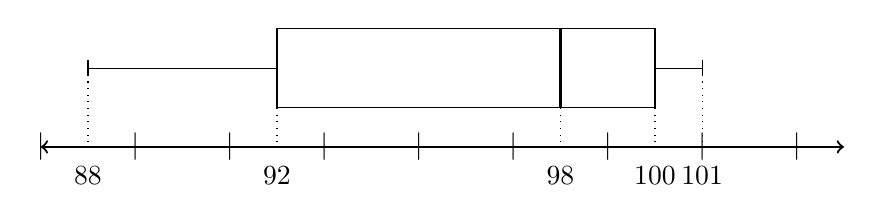
\begin{tikzpicture}[xscale=0.6]
      \def\median{98}
      \def\firstquartile{92}
      \def\thirdquartile{100}
      \def\minimum{88}
      \def\maximum{101}
      \draw (\firstquartile, -0.5 ) rectangle ( \thirdquartile,0.5);
      \draw[thick] ( \median,-0.5) -- ( \median,0.5);
      \draw (    \firstquartile, 0) -- (\minimum,0   );
      \draw ( \minimum, -0.1) -- (       \minimum, 0.1);
      \draw (  \thirdquartile, 0) -- (   \maximum, 0);
      \draw ( \maximum, -0.1) -- (      \maximum, 0.1 );
      \draw[thick,<->] (87,-1) -- (104,-1);
      \foreach \x in {\minimum, \firstquartile, \median, \thirdquartile, \maximum} {
        \draw (\x,-1.6) -- (\x, -1.6) node[anchor=south] {$\x$};
      }
      \foreach \x in {87,89,...,104} {
        \draw (\x,-1.3) -- (\x, -1.3) node[anchor=south] {$|$};
      }
      \draw[dotted] ( \maximum, 0) -- ( \maximum, -1);
      \draw[dotted] ( \thirdquartile, 0) -- ( \thirdquartile, -1);
      \draw[dotted] (\median, 0)  -- ( \median, -1);
      \draw[dotted] (\firstquartile, 0) -- ( \firstquartile, -1);
      \draw[dotted] ( \minimum, 0) -- ( \minimum, -1);
    \end{tikzpicture}
\end{enumerate}
\end{enumerate}
}
\end{exercises}


 \begin{solutions}{}{
\begin{enumerate}[itemsep=5pt, label=\textbf{\arabic*}. ] 


\item \\%solution 1
Minimum: $3$ \\
$Q_1$: $17,5$ \\
Median: $27$\\
$Q_3$: $44$\\
Maximum: $65$\\
\par
\scalebox{0.8}{
    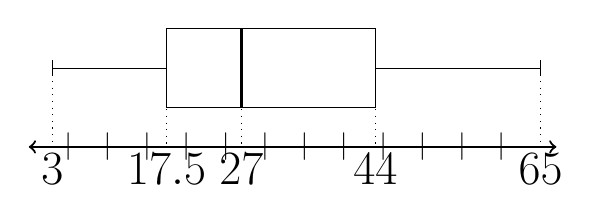
\begin{tikzpicture}[xscale=0.1]
      \def\median{27}
      \def\firstquartile{17.5}
      \def\thirdquartile{44}
      \def\minimum{3}
      \def\maximum{65}

      \draw (\firstquartile, -0.5 ) rectangle ( \thirdquartile,0.5);
      \draw[thick] ( \median,-0.5) -- ( \median,0.5);
      \draw (    \firstquartile, 0) -- (\minimum,0   );
      \draw ( \minimum, -0.1) -- (       \minimum, 0.1);
      \draw (  \thirdquartile, 0) -- (   \maximum, 0);
      \draw ( \maximum, -0.1) -- (      \maximum, 0.1 );

      \draw[thick,<->] (0,-1) -- (67,-1);

      \foreach \x in {\minimum, \firstquartile, \median, \thirdquartile, \maximum} {
        \draw (\x,-1.6) -- (\x, -1.6) node[anchor=south] {\LARGE $\x$};
      }

      \foreach \x in {5,10,...,60} {
        \draw (\x,-1.3) -- (\x, -1.3) node[anchor=south] {$|$};
      }
      \draw[dotted] ( \maximum, 0.09) -- ( \maximum, -1);
      \draw[dotted] ( \thirdquartile, 0.49) -- ( \thirdquartile, -1);
      \draw[dotted] (\median, 0.49)  -- ( \median, -1);
      \draw[dotted] (\firstquartile, 0.49) -- ( \firstquartile, -1);
      \draw[dotted] ( \minimum, 0.09) -- ( \minimum, -1);
    \end{tikzpicture}}

\item %solution 2
Minimum: $1$ \\
$Q_1$: $12$ \\
Median: $28,5$\\
$Q_3$: $46,5$\\
Maximum: $60$\\
\par
%   sales.
\scalebox{0.8}{
    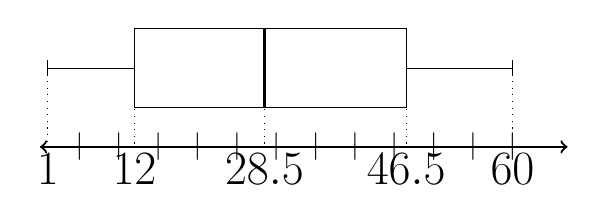
\begin{tikzpicture}[xscale=0.1]
      \def\median{28.5}
      \def\firstquartile{12}
      \def\thirdquartile{46.5}
      \def\minimum{1}
      \def\maximum{60}

      \draw (\firstquartile, -0.5 ) rectangle ( \thirdquartile,0.5);
      \draw[thick] ( \median,-0.5) -- ( \median,0.5);
      \draw (    \firstquartile, 0) -- (\minimum,0   );
      \draw ( \minimum, -0.1) -- (       \minimum, 0.1);
      \draw (  \thirdquartile, 0) -- (   \maximum, 0);
      \draw ( \maximum, -0.1) -- (      \maximum, 0.1 );

      \draw[thick,<->] (0,-1) -- (67,-1);

      \foreach \x in {\minimum, \firstquartile, \median, \thirdquartile, \maximum} {
        \draw (\x,-1.6) -- (\x, -1.6) node[anchor=south] {\LARGE $\x$};
      }

      \foreach \x in {5,10,...,60} {
        \draw (\x,-1.3) -- (\x, -1.3) node[anchor=south] {$|$};
      }
      \draw[dotted] ( \maximum, 0.09) -- ( \maximum, -1);
      \draw[dotted] ( \thirdquartile, 0.49) -- ( \thirdquartile, -1);
      \draw[dotted] (\median, 0.49)  -- ( \median, -1);
      \draw[dotted] (\firstquartile, 0.49) -- ( \firstquartile, -1);
      \draw[dotted] ( \minimum, 0.09) -- ( \minimum, -1);
    \end{tikzpicture}}
\item %solution 3
Minimum: $3$ \\
$Q_1$: $5$ \\
Median: $7$\\
$Q_3$: $13$\\
Maximum: $16$\\
\item %solution 4
 \begin{enumerate}[itemsep=5pt, label=\textbf{(\alph*)} ]
\item \\
Minimum: $15$ \\
$Q_1$: $22$ \\
Median: $25$\\
$Q_3$: $28$\\
Maximum: $35$\\

\item \\%
Minimum: $88$ \\
$Q_1$: $92$ \\
Median: $98$\\
$Q_3$: $100$\\
Maximum: $101$\\   
\end{enumerate}
\end{enumerate}}
\end{solutions}


\begin{eocexercises}{}
  \begin{enumerate}[itemsep=6pt, label=\textbf{\arabic*}.]
  \item 
  In a park, the tallest $7$ trees have heights in metres of
    $41$; $60$; $47$; $42$; $44$; $42$; and $47$. Find the median of
    their heights.
  \item The students in Ndeme's class have the following ages: $5$;
    $6$; $7$; $5$; $4$; $6$; $6$; $6$; $7$; $4$. Find the mode of
    their ages.
  \item An engineering company has designed two different types of
    engines for motorbikes. The two different motorbikes are tested
    for the time (in seconds) it takes for them to accelerate from $0$
    km/h to $60$ km/h.
    \begin{center}
      \begin{tabular}{|@{\hspace{0.1cm}}c@{\hspace{0.1cm}}|@{\hspace{0.1cm}}c@{\hspace{0.1cm}}|@{\hspace{0.1cm}}c@{\hspace{0.1cm}}|@{\hspace{0.1cm}}c@{\hspace{0.1cm}}|@{\hspace{0.1cm}}c@{\hspace{0.1cm}}|@{\hspace{0.1cm}}c@{\hspace{0.1cm}}|@{\hspace{0.1cm}}c@{\hspace{0.1cm}}|@{\hspace{0.1cm}}c@{\hspace{0.1cm}}|@{\hspace{0.1cm}}c@{\hspace{0.1cm}}|@{\hspace{0.1cm}}c@{\hspace{0.1cm}}|@{\hspace{0.1cm}}c@{\hspace{0.1cm}}|} \hline
        & \textbf{Test 1} & \textbf{Test 2} & \textbf{Test 3} & \textbf{Test 4} & \textbf{Test 5} & \textbf{Test 6} & \textbf{Test 7} &\textbf{Test 8} & \textbf{Test 9} & \textbf{Test 10} \\\hline
        \textbf{Bike 1} & $1,55$ & $1,00$ & $0,92$ & $0,80$ & $1,49$ & $0,71$ & $1,06$ & $0,68$ & $0,87$ & $1,09$ \\\hline
        \textbf{Bike 2} & $0,9$ & $1,0$ & $1,1$ & $1,0$ & $1,0$ & $0,9$ & $0,9$ & $1,0$ & $0,9$ & $1,1$ \\\hline
      \end{tabular}
    \end{center}
\vspace {8pt}\\
\begin{enumerate}[noitemsep, label=\textbf{(\alph*)} ]
    \item Which measure of central tendency should be used for this
      information?
    \item Calculate the measure of central tendency that you chose in
      the previous question, for each motorbike.
    \item Which motorbike would you choose based on this information?
      Take note of the accuracy of the numbers from each set of tests.
    \end{enumerate}
  \item In a traffic survey, a random sample of $50$ motorists were
    asked the distance they drove to work daily. This information is
    shown in the table below.\\
    \begin{center}
      \begin{tabular}{|c|c|} \hline
        \textbf{Distance (km)} & \textbf{Count} \\ \hline
        $0 < d \leq 5$ & $4$ \\ \hline
        $5 < d \leq 10$ & $5$ \\\hline
        $10 < d \leq 15$ & $9$ \\\hline
        $15 < d \leq 20$ & $10$ \\\hline
        $20 < d \leq 25$ & $7$ \\\hline
        $25 < d \leq 30$ & $8$ \\\hline
        $30 < d \leq 35$ & $3$ \\\hline
        $35 < d \leq 40$ & $2$ \\\hline
        $40 < d \leq 45$ & $2$ \\\hline
      \end{tabular}
    \end{center}
\vspace {8pt}\\
     \begin{enumerate}[noitemsep, label=\textbf{(\alph*)} ]
    \item Find the approximate mean of the data.
    \item What percentage of samples had a distance of
      \begin{enumerate}[noitemsep, label=\textbf{\roman*}. ]
      \item less than $16$ km?
      \item more than $30$ km?
      \item between $16$ km and $30$ km daily?
      \end{enumerate}
\item Draw a histogram to represent the data
    \end{enumerate}
  \item A company wanted to evaluate the training programme in its
    factory. They gave the same task to trained and untrained
    employees and timed each one in seconds.
\\
    \begin{center}
      \begin{tabular}{|l|c|c|c|c|c|} \hline
        \textbf{Trained} & 121 & 137 & 131 & 135 & 130 \\ \hline
                         & 128 & 130 & 126 & 132 & 127 \\\hline
                         & 129 & 120 & 118 & 125 & 134 \\\hline
        \textbf{Untrained} & 135 & 142 & 126 & 148 & 145 \\\hline
                           & 156 & 152 & 153 & 149 & 145 \\\hline
                           & 144 & 134 & 139 & 140 & 142 \\\hline
      \end{tabular}
    \end{center}
\vspace {8pt}\\
    \begin{enumerate}[noitemsep, label=\textbf{(\alph*)} ]
    \item Find the medians and quartiles for both sets of data.
    \item Find the interquartile range for both sets of data.
    \item Comment on the results.
    \item Draw a box-and-whisker diagram for each data set to illustrate the five number summary.
    \end{enumerate}
  \item A small firm employs nine people. The annual salaries of the employers are:
\\
    \begin{center}
      \begin{tabular}{|r|r|r|} \hline
        R $600~ 000$ & R $250~ 000$ & R $200~ 000$ \\\hline
        R $120 ~000 $& R $100~ 000$ & R $100 ~000$ \\\hline
        R $100 ~000$ & R  $90~ 000$ & R  $80 ~000$ \\\hline
      \end{tabular}
    \end{center}
\vspace {8pt}\\
    \begin{enumerate}[noitemsep, label=\textbf{(\alph*)} ]
    \item Find the mean of these salaries.
    \item Find the mode.
    \item Find the median.
    \item Of these three figures, which would you use for
      negotiating salary increases if you were a trade union
      official? Why?
    \end{enumerate}
  \end{enumerate}

\end{eocexercises}


\begin{eocsolutions}{}{
\begin{enumerate}[itemsep=5pt, label=\textbf{\arabic*}. ] 
\item %solution 1
Median $=\dfrac{41+60+47+42+44+42+47}{7} \\
~~~~~~~~=44$
\item %solution 2
Mode $=6$
\item %solution 3
  \begin{enumerate}[noitemsep, label=\textbf{(\alph*)} ]
  \item Mean and Mode. The mean will give us the average acceleration time, while the mode will give us the time that is most often obtained.%What measure of central tendency should be used for this
    % information?
  \item For bike $1$ the mean is $1,02$ s and no mode, since there is no value that occurs more than once.\\
    For bike $2$ the mean is $1,0$ s and there are two modes, $1,0$ and $0,9$.
  \item It would be difficult to choose. Although bike $1$ appears to do better than bike $2$ from the mean, the data for bike $2$ is less accurate than that for bike $1$ (it only has $1$ decimal place.) If we were to calculate the mean for bike $1$ using only $1$ decimal place we would get $0,9$ s. This would make bike $2$ better. Also bike $2$ produces more consistent numbers. So bike $2$ would likely be a good choice, but more information or more accurate information should be obtained.
  \end{enumerate}

\item %solution 4
  \begin{enumerate}[noitemsep, label=\textbf{(\alph*)} ]
  \item Mean $=\dfrac{4(3)+5(8)+9(13)+10(18)+7(23)+8(28)+3(33)+2(38)+2(43)}{50}\\
~~~~~~=19,9$
  \item %What percentage of samples had a speed of
    \begin{enumerate}[noitemsep, label=\textbf{\roman*}. ]
    \item There were $18$ drivers who drove less than $15$ km.\\
      Therefore $\frac{18}{50}\times 100 = 38\%$%less than $15$ km?
    \item There were $7$ drivers who drove less than $30$ km.\\
      Therefore $\frac{7}{50}\times 100 = 14\%$%more than $30$ km?
    \item $100-(36-14) = 50\%$%between $16$ km and $30$ km daily?
    \end{enumerate}
  \item %Draw a histogram to represent the data
\scalebox{0.8} % Change this value to rescale the drawing.
{
\begin{pspicture}(0,-3.62375)(11.17442,3.58375)
\definecolor{color6331b}{rgb}{0.7725490196078432,0.7725490196078432,0.7725490196078432}
\psframe[linewidth=0.02,dimen=outer,fillstyle=solid,fillcolor=color6331b](2.208587,-0.41625)(1.1885868,-2.4128125)
\rput(1.1744202,-2.41625){\psaxes[linewidth=0.028222222,arrowsize=0.05291667cm 2.0,arrowlength=1.4,arrowinset=0.4,tickstyle=bottom,ticksize=0.10583333cm,dx=1.0cm,dy=0.5cm,Dx=5]{<->}(0,0)(-1,-1)(10,6)}
\psframe[linewidth=0.02,dimen=outer,fillstyle=solid,fillcolor=color6331b](3.188587,0.10375)(2.168587,-2.4128125)
\psframe[linewidth=0.02,dimen=outer,fillstyle=solid,fillcolor=color6331b](4.2085867,2.10375)(3.168587,-2.4128125)
\psframe[linewidth=0.02,dimen=outer,fillstyle=solid,fillcolor=color6331b](5.2085867,2.60375)(4.1685867,-2.4128125)
\psframe[linewidth=0.02,dimen=outer,fillstyle=solid,fillcolor=color6331b](6.1885867,1.12375)(5.1685867,-2.4128125)
\psframe[linewidth=0.02,dimen=outer,fillstyle=solid,fillcolor=color6331b](7.1885867,1.58375)(6.1685867,-2.4128125)
% \usefont{T1}{ptm}{m}{n}
\rput(6.062962,-3.42625){\LARGE Distance (km)}
% \usefont{T1}{ptm}{m}{n}
\rput{89.854546}(1.2403736,0.9631185){\rput(0.11709099,1.0822288){\LARGE Count}}
\psframe[linewidth=0.02,dimen=outer,fillstyle=solid,fillcolor=color6331b](8.188587,-0.89625)(7.1685867,-2.4128125)
\psframe[linewidth=0.02,dimen=outer,fillstyle=solid,fillcolor=color6331b](9.188587,-1.39625)(8.168587,-2.4128125)
\psframe[linewidth=0.02,dimen=outer,fillstyle=solid,fillcolor=color6331b](10.188587,-1.39625)(9.168587,-2.4128125)
\end{pspicture} 
}
  \end{enumerate}

\item %solution 5
  \begin{enumerate}[noitemsep, label=\textbf{(\alph*)} ]
  \item First order the data sets for both trained and untrained employees.\\
    Trained: $118, 120, 121, 125, 126, 127, 128, 129, 130, 130, 131, 132, 134, 135, 137$ \\
    Untrained: $126, 134, 135, 139, 140, 142, 142, 144, 145, 145, 148, 149, 152, 153, 156$ \\
    There are $15$ values in each data set. \\
    Position of the median is $\frac{15+1}{2}=8$. \\
    For the trained employees this is $129$ and for the untrained employees this is $144$.\\
    Positions of the quartiles are $\frac{15}{4}=3,75$.\\
    For the trained employees: $Q_1=125$ and $Q_3=132$.\\
    For the untrained employees: $Q_1=139$ and $Q_3=149$.\\
  \item
    Interquartile range for the trained employees: $Q_3-Q_1=7$.\\
    Interquartile range for the untrained employees: $Q_3-Q_1=10$.\\
  \item
    The median of the untrained employees is higher than that of the trained employees. Also the untrained employees have a larger interquartile range than the trained employees. There is some evidence to suggest that the training programme may be working.
  \item %Draw two box-and-whisker diagrams to illustrate the five number summary
    Trained employees:\\
\scalebox{1}{
    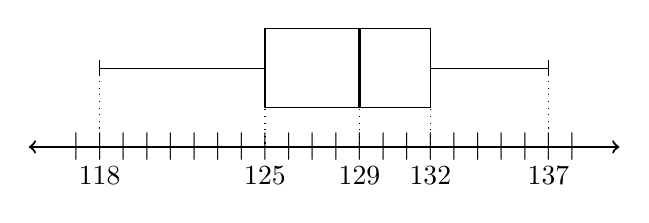
\begin{tikzpicture}[xscale=0.3]
      \def\median{129}
      \def\firstquartile{125}
      \def\thirdquartile{132}
      \def\minimum{118}
      \def\maximum{137}

      \draw (\firstquartile, -0.5 ) rectangle ( \thirdquartile,0.5);
      \draw[thick] ( \median,-0.5) -- ( \median,0.5);
      \draw (    \firstquartile, 0) -- (\minimum,0   );
      \draw ( \minimum, -0.1) -- (       \minimum, 0.1);
      \draw (  \thirdquartile, 0) -- (   \maximum, 0);
      \draw ( \maximum, -0.1) -- (      \maximum, 0.1 );

      \draw[thick,<->] (115,-1) -- (140,-1);

      \foreach \x in {\minimum, \firstquartile, \median, \thirdquartile, \maximum} {
        \draw (\x,-1.6) -- (\x, -1.6) node[anchor=south] {$\x$};
      }

      \foreach \x in {117,118,...,138} {
        \draw (\x,-1.3) -- (\x, -1.3) node[anchor=south] {$|$};
      }
      \draw[dotted] ( \maximum, 0.09) -- ( \maximum, -1);
      \draw[dotted] ( \thirdquartile, 0.49) -- ( \thirdquartile, -1);
      \draw[dotted] (\median, 0.49)  -- ( \median, -1);
      \draw[dotted] (\firstquartile, 0.49) -- ( \firstquartile, -1);
      \draw[dotted] ( \minimum, 0.09) -- ( \minimum, -1);
    \end{tikzpicture}}
  
\\
Untrained employees:\\
\scalebox{1}{
    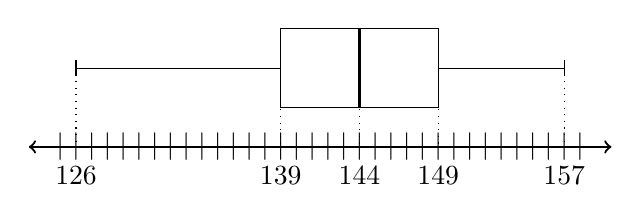
\begin{tikzpicture}[xscale=0.2]
      \def\median{144}
      \def\firstquartile{139}
      \def\thirdquartile{149}
      \def\minimum{126}
      \def\maximum{157}

      \draw (\firstquartile, -0.5 ) rectangle ( \thirdquartile,0.5);
      \draw[thick] ( \median,-0.5) -- ( \median,0.5);
      \draw (    \firstquartile, 0) -- (\minimum,0   );
      \draw ( \minimum, -0.1) -- (       \minimum, 0.1);
      \draw (  \thirdquartile, 0) -- (   \maximum, 0);
      \draw ( \maximum, -0.1) -- (      \maximum, 0.1 );

      \draw[thick,<->] (123,-1) -- (160,-1);

      \foreach \x in {\minimum, \firstquartile, \median, \thirdquartile, \maximum} {
        \draw (\x,-1.6) -- (\x, -1.6) node[anchor=south] {$\x$};
      }

      \foreach \x in {125,126,...,158} {
        \draw (\x,-1.3) -- (\x, -1.3) node[anchor=south] {$|$};
      }
      \draw[dotted] ( \maximum, 0.09) -- ( \maximum, -1);
      \draw[dotted] ( \thirdquartile, 0.49) -- ( \thirdquartile, -1);
      \draw[dotted] (\median, 0.49)  -- ( \median, -1);
      \draw[dotted] (\firstquartile, 0.49) -- ( \firstquartile, -1);
      \draw[dotted] ( \minimum, 0.09) -- ( \minimum, -1);
    \end{tikzpicture}}
  \end{enumerate}
\item %solution 6
  \begin{enumerate}[noitemsep, label=\textbf{(\alph*)} ]
  \item
    Mean $=\frac{1~640~000}{9}=182~222,22$
  \item
    Mode is R $100~000$.
  \item
    First order the data. To make the numbers easier to work with we will divide each one by $100~000$.\\
    The ordered set is $80, 90, 100, 100, 100, 120, 200, 250, 600$.  \\
    The median is at position $5$ and is R $100~000$.
  \item
    Either the mode or the median. \\
    The mean is skewed (shifted) by the one salary of R $600~000$. The mode gives us a better estimate of what the employees are actually earning. The median also gives us a fairly accurate representation of what the employees are earning.
  \end{enumerate}
\end{enumerate}
}
\end{eocsolutions}


